\documentclass[./dissertation.tex]{subfiles}
\begin{document}


\chapter{Failure Mode and Effect Analysis FMEA}

\section{Introduction}
\subsection{General}
FMEA and FMECA are important techniques for a reliability assurance programme.They can be applied to a wide range of problems which may occur in technical systems, and can be carried out in varying degrees of depth, or modified, to suit a particular purpose. The analysis is carried out in a limited way during the conception, planning, and definition phases and more fully in the design and development phase. It is however important to remember that the FMEA is only part of a reliability and
maintainability programme which requires many different tasks and activities. FMEA is an inductive method of performing a qualitative system reliability or safety analysis from a low to a high level. A thorough understanding of the system under analysis is essential prior to undertaking FMEA. Functional diagrams and other system drawings are normally necessary for this understanding. Reliability block diagrams, fault trees and/or state diagrams are then usually derived from these in order to
carry out the analysis. In many instances the block diagram descriptions and block diagram failure descriptions are included in the FMEA format. Separate diagrams will be needed for the
following:
\begin{enumerate}
    \item The way in which different criteria for system failure are determined;
    \item Degradation of function or reduction in assurance of function;
    \item Alternative operational phases
\end{enumerate}

\subsection{Purpose of the Analysis}
The reasons for undertaking FMEA (or FMECA) may include the following:

\begin{itemize}
    \item to identify those failures which have unwanted effects on system operation, e.g. safety critical failures;
    \item to satisfy contractual conditions that an FMEA should be completed;
    \item where appropriate, to quantify the reliability and/or safety of the system;
    \item to allow improvements of the system's reliability and/or safety (e.g. by design or quality assurance action)
    \item to produce aids to fault diagnosis;
    \item to allow improvement of the system's maintainability (by highlighting areas of risk or non-conformance for maintainability).
\end{itemize}

ln view of these reasons the objectives of an FMEA (or FMECA) may include the following: 

\begin{enumerate}
    \item a comprehensive identification and evaluation of all the unwanted effects within the defined boundaries of the system being analysed, and the sequences of events brought about by each identified item failure mode, from whatever cause, at various levels of the system's functional hierarchy;
    \item the determination of the significance (or criticality) of each failure mode with respect to the system's correct function or performance and the impact on the reliability and/or safety of the process concerned;
    \item a classification of identified failure modes according to relevant characteristics, including detectability, diagnosability, testability, item replaceability, compensating and operating provisions (repair, maintenance, logistics, etc.);
    \item an estimation of measures of the significance and probability of failure.
\end{enumerate}


\subsection{Basic Principles of FMEA}
The following concepts are essential to FMEA:

\begin{enumerate}
    \item breakdown of the system into 'elements';
    \item a diagram of the system's functional structure and identification of the various data which are needed to perform the FMEA;
    \item the failure mode concept (a part may have several failure modes or a failure mode may involve several parts);
    \item identification of new physical features or new requirements;
    \item the criticality concept and the measure to be used (if criticality analysis is required).
\end{enumerate}

Further, it is essential to specify the existing links between the FMEA (and the FMECA) and other qualitative (and quantitative) analytical methods within the overall reliability programme.  Very few designs are wholly new. Most are to some extent developments of old designs. FMEA should use the information on existing systems and draw attention to the need for tests, etc. for the new parts.  



\section{Procedure}

\subsection{General}
The wide variation in complexity of system designs and applications may require the development of highly individualised FMEA procedures consistent with the information available. Traditionally, there have been wide variations in the manner in which FMEA is conducted and presented. However, the analysis is usually done in a standard manner and presented on a worksheet that contains a core of essential information which can be developed and extended to suit the particular system or project to which it is applied. A typical example of a worksheet is shown in Figure 1.

The procedure consists of the following four main stages:

\begin{enumerate}
\item Preparatory definition of the system including the design, functional, operational, maintenance, and environmental requirements;
\item Establishment of the basic principles and purposes of the FMEA and the form of its presentation;
\item Carrying out the FMEA using the appropriate worksheet designed according to (a) and (b);
\item Reporting of the complete analysis including any conclusions and recommendations made.
\end{enumerate}

A more detailed consideration of the information needed is given in the following sections.

\subsection{Preparation}
At the commencement of an analysis, the following preparations should be made:
\begin{enumerate}
\item The analyst should have available the information listed in Section 2.4.2.2 to 2.4.2.7 that clearly defines the system to be analysed.
\item It will usually be necessary for the analyst to translate the information into some form of functional, hierarchical, or reliability block diagrams. An example of a functional diagram is shown in Figure 2. This diagram shows how the failure effects at the part level form the failure modes at the module level, the failure effects at the module level form the failure modes at the subsystem level, and so on. Such a representation of the system should explicitly identify the system's functional structure, the system boundary, and the inputs and outputs crossing that boundary. Further information is given in Section 2.4.2.8 to 2.4.2.10.
\end{enumerate}

\subsection{FMEA principles}
The following principles should be applied:
\begin{enumerate}
\item Define clearly the purposes and uses of the FMEA as indicated in Section 2.1.2.
\item Establish and define the relationships with other forms of reliability analysis with which the FMEA may subsequently be integrated. (See Section 2.3.5.)
\item Define the scope of the FMEA in relation to the functional structure and hierarchical structure of the system as described by the block diagrams referred to in Section 2.4.2.10. It is essential to define the lowest level in the system's hierarchical structure at which the analysis will start. The guidance given in Sections 2.3.4, 2.4.1, and 2.4.2.8 is especially important for this task.
\item Define the format of the FMEA worksheet to suit the project requirements. The core information considered essential is as follows:
\end{enumerate}

\begin{enumerate}
\item The name of the item in the system being analysed;
\item Function performed by the item;
\item Identification number of the item;
\item Failure modes of the item;
\item Failure causes;
\item Failure effects on the system;
\item Failure detection methods;
\item Compensating provisions;
\item Severity of effects;
\item Remarks.
\end{enumerate}
Other information required for the particular system and project needs to be defined by the analyst according to the purposes of the



\section{Analysis}
It is worth to underline that, even though the scope of this thesis is to establish a new methodology for automated FMEA in both hardware and software systems, there is the absolute need to comply with what is today the state of the art for FMEA and the guidelines to be followed to bring the metrics extracted during the analysis to certification. It is for this reason that the following section will present the traditional method applied today to all the electromechanical systems under evaluation. Bare in mind that the totality of the procedure described below is man driven.

The usual requirement and purpose of an FMEA is to identify the effect of oJl failure modes of all constituent items at the lowest level in the system.Tb achieve this the worksheet should be used in the following manner:

\begin{enumerate}

	\item Identify all items in the system or subsystem,each of which is to have its failure modes and effects analysed. The system of identification by name and number should be such that no item swill be omitted.
	\item Select the first item for analysis and enter the item name and identification number in the appropriate columns of the worksheet.Determine the function of that item in the system and enter that on the worksheet.
	\item Deduce all the possible failure modes of the item due to any possible cause and individually enter these modes on the worksheet
	\item  Postulate the most likely failure causes for each failure mode of the item and enter these on the worksheet. It will usually not be possible to consider all possible causes because the range is so vast, but the most significant with regard to the item, the failure mode and the application should be identified.
	\item Deduce the effects of the failure on the subsystem and system, as determined by the scope of the FMEA
	\item  Complete the remaining columns of the worksheet for the first failure mode of the first item.
	\item Repeat 3 to 5 for all failure modes of the first item
	\item Repeat 2 to 6 for all other items
\end{enumerate}


\subsection{Multiple Stages}
If the FMEA is to be done in stages that each relate to separate Levels in the system's hierarchical structure, the failure effects from the lower level become the failure modes at the next level up. The analysis should then proceed as follows.

\begin{enumerate}
	\item Identify the lower level FMEAs that are appropriate for the next stage in the system FMEA according to the system's hierarchical structure defined by the block or functional diagrams (see 2.2,2(b)). Where appropriate also include items defined as being at the lowest level in that part of the system structure
	\item Perform the FMEA for each failure of each item at this higtrer level in the system structures given in the previous section.
	\item repeat the two above steps for any further higher levels in the system structure.
\end{enumerate}
\subsection{Worksheet recommendations}

The last worksheet entry should give any pertinent remarks to clarify other entries. Possible future actions such as recommendations for design improvements may be recorded and then amplified in the report. This column may also include the following:

\begin{enumerate}
\item[(a)] any unusual conditions;
\item[(b)] effects of redundant element failures;
\item[(c)] recognition of specially critical design features;
\item[(d)] any remarks to amplify the entry;
\item[(e)] references to other entries for sequential failure analysis;
\item[(f)] significant maintenance requirements;
\item[(g)] dominant failure causes;
\item[(h)] dominant failure effects;
\item[(i)] decisions taken, e.g. at design review.
\end{enumerate}


The report on the FMEA (or FMECA) may be included in a wider study or may stand alone. In neither case, the report should include a summary and a detailed record of the analysis and the block or functional diagrams which define the system structure. The report should also contain a list of the drawings (including issue status) on which the FMEA is based.

The summary should contain a brief description of the method of analysis and the level to which it was conducted, the assumptions and the ground rules. In addition, it should include listings of the following:

\begin{enumerate}
\item recommendations for the attention of designers, maintenance staff, planners, and users;
\item failures which, when initially occurring alone, result in serious effects;
\item failures which have no effect;
\item design changes which have already been incorporated as a result of the FMEA (or FMECA).
\end{enumerate}



\begin{figure}
        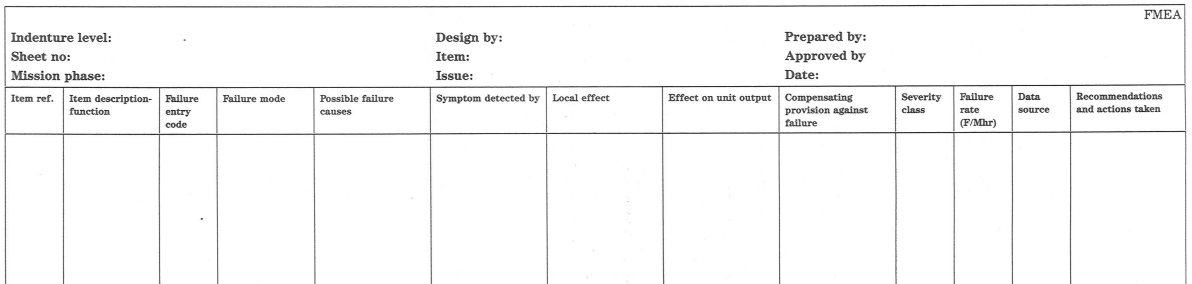
\includegraphics[width=\linewidth]{subfiles/imgs/FMEA_table.png}
  \caption{Example of FMEA Table}
        \label{fig:fmea_table}
\end{figure}


\begin{figure}
        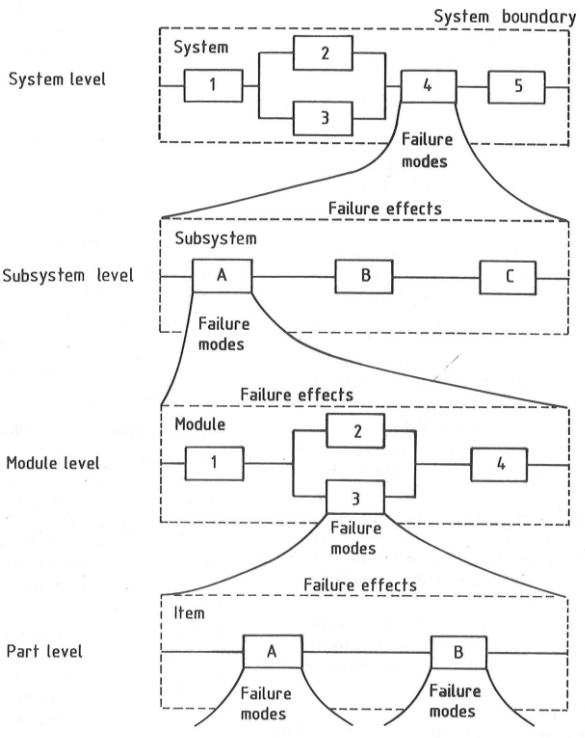
\includegraphics[width=\linewidth]{subfiles/imgs/fmea_relationship_failure_mode_effects.png}
  \caption{Criticality Grid}
        \label{fig:criticality_grid}
\end{figure}


\subsection{Report on Analysis}

The report on Failure Modes and Effects Analysis (FMEA) or Failure Modes, Effects and Criticality Analysis (FMECA) can be either a standalone document or a part of a broader study. In either case, the report should contain a summary and a detailed record of the analysis along with block or functional diagrams that define the structure of the system. Furthermore, the report should include a list of drawings (with issue status) on which the FMEA is based.

The summary section of the report should provide a brief explanation of the analysis method, the level to which it was carried out, the assumptions made, and the ground rules followed (see section 2.4.L). The summary should also include lists of the following:

\begin{enumerate}
\item Recommendations for designers, maintenance staff, planners, and users;
\item Failures that, when occurring alone, have significant consequences;
\item Failures that have no impact; and
\item Design changes that were made as a result of the FMEA (or FMECA).
\end{enumerate}



\section{Application}
\subsection{Field of application}
FMEA is a method that is primarily adapted to the study of material and equipment failures and that can be applied to categories of systems based on different technologies (electrical, mechanical, hydraulic, etc.) and combinations of technologies. FMEA should also include the consideration of software and human performance where these are relevant to the reliability of the system. An FMEA can be a study for general use or it may be specific to particular pieces of equipment, to systems or to projects as a whole.

\subsection{Application within a project}
The user should determine how and for what purposes he uses FMEA within his own technical discipline. It may be used alone or to complement and support other methods of reliability analysis. The requirements for FMEA originate from the need to understand hardware behaviour and its implications for the operation of the system or equipment. The need for FMEA can vary widely from one project to another. FMEA is the principal reliability engineering activity in support of the design review concept (see 4.2.1.4 of BS 5760: Part 1: 1988) and should be put into use from the very first steps of system and subsystem design. FMEA is applicable to all levels of system design but is most appropriate for lower levels where large numbers of items are involved and/or there is functional complexity. Special training of personnel performing FMEA is essential and they need the close collaboration of systems engineers and designers. The FMEA should be updated as the project progresses and as designs are modified. At the end of the project, FMEA is used to check the design and may be essential for demonstration of conformity of a designed system to the required standards, regulations, and user's requirements.

Information from the FMEA identifies priorities for statistical process control sampling and inspection tests during manufacture and installation and for qualification, approval, acceptance and start-up tests. It provides essential information for diagnostic and maintenance procedures for inclusion in handbooks.

In deciding on the extent and the way in which FMEA should be applied to an item or design, it is important to consider the specific purposes for which FMEA results are needed, the time phasing with other activities and the importance of establishing a predetermined degree of awareness and control over unwanted failure modes and effects. This leads to the planning of FMEA in qualitative terms at specified levels (system, subsystem, component, item) to relate to the iterative design and development process (see BS 5760: Part 1).

To ensure that it is effective, the place of FMEA should be clearly established in the reliability program, together with the time, manpower and other resources needed to make it effective. It is vital that FMEA is not abridged to save time and money. If time and money are short the FMEA should concentrate on those parts of the design which are new or are used in new ways. FMEA can be economically directed to areas identified as crucial by other methods of analysis, e.g. fault tree analysis (FTA).


\subsection{Uses of FMEA}

Some of the detailed applications and benefits of FMEA are listed below:

\begin{enumerate}
\item[(a)] to avoid costly modifications by the early identification of design deficiencies;
\item[(b)] to identify failures which, when they occur alone or in combination, have unacceptable or significant effects, and to determine the failure modes which may seriously affect the expected or required operation; \footnote{Such effects may include secondary failures.}
\item[(c)] to determine the need for the following:
\begin{enumerate}
\item[(1)] redundancy;
\item[(2)] design improvement;
\item[(3)] more generous stress allowances (derating);
\item[(4)] screening of items;
\item[(5)] design of features that ensure that the system fails in a preferred failure mode, e.g. 'fail-safe' outcomes of failures;
\item[(6)] selection of alternative materials, parts, devices, and components;
\end{enumerate}
\item[(d)] to identify serious failure consequences and hence the need for changes in design and/or operational rules;
\item[(e)] to provide the logic model required to evaluate the probability or rate of occurrence of anomalous operating conditions of the system in preparation for criticality analysis;
\item[(f)] to disclose safety hazard, and product liability problem areas, or non-compliance with regulatory requirements; \textbf{Note:} Frequently, separate studies will be required for safety, but overlap is inevitable and therefore cooperation is highly advisable.
\item[(g)] to ensure that the development test programme can detect potential failure modes;
\item[(h)] to focus upon key areas in which to concentrate quality control, inspection and manufacturing process controls;
\item[(i)] to assist in defining various aspects of the general maintenance strategy, such as:
\begin{enumerate}
\item[(1)] establishing the need for data recording and condition monitoring during testing, checking-out and use;
\item[(2)] provision of information for development of trouble-shooting guides;
\item[(3)] establishing maintenance cycles which anticipate and avoid wear-out failures;
\item[(4)] the selection of preventative or corrective maintenance schedules, facilities, equipment and staff;
\item[(5)] selection of built-in test equipment and suitable test points;
\end{enumerate}
\item[(j)] to provide a systematic and rigorous approach to the study of the installation in which the system is embedded;
\item[(k)] to facilitate or support the determination of test criteria, test plans and diagnostic procedures, for example: performance testing, reliability testing;
\item[(l)] to identify parts and assemblies requiring worst case analysis (frequently required for failure modes involving parameter drifts);
\item[(m)] to support the design of fault isolation sequences and to support the planning for alternative modes of operation and reconfiguration;
\item[(n)] to facilitate communication between the following:
\begin{enumerate}
\item[(1)] general and specialised engineers;
\item[(2)] equipment manufacturer and his suppliers;
\item[(3)] system user and the designer or manufacturer;
\end{enumerate}
\item[(o)] to enhance the analyst's knowledge and understanding of the behaviour of the equipment studied;
\item[(p)] to provide designers with an understanding of the factors which influence the reliability of the system;
\item[(q)] to provide a final document that is proof of the fact that (and of the extent to which) care has been taken to ensure that the design will meet its specification in service. (This is especially important in the case of product liability 
\end{enumerate}



\subsection{Limitations and Drawbacks}
FMEA is extremely efficient when it is applied to the analysis of elements that cause a failure of the entire system or of a major function of the system. However, FMEA may be difficult and tedious for the case of complex systems that have multiple functions involving different sets of system components. This is because of the quantity of detailed system information that needs to be considered. This difficulty can be increased by the existence of a number of possible operating modes, as well as by consideration of the repair and maintenance policies. FMEA can be a laborious and inefficient process unless it is judiciously applied. The uses to which the results are to be put subsequently should be defined and FMEA should not be included in requirements specifications indiscriminately. Complications, misunderstandings and errors can occur when FMEA attempts to span several levels in a hierarchical structure if redundancy is applied in the system design. It is therefore preferable for an FMEA to be restricted to relating two levels only in the hierarchical structure. For example, it is a relatively straightforward task to identify failure modes of items and to determine their effects on the assembly. These effects then become the failure modes at the next level up, e.g. the module, and so on. However, successful multi-level FMEAs are often carried out. FMEA is applicable to all levels of a system but is most appropriate to lower levels where large numbers of items are involved and/or there is functional complexity.

\subsection{Relationships with Other Methods}
FMEA (or FMECA) can be used alone. As a systematic inductive method of analysis, FMEA is most often used to complement other approaches, especially deductive ones. At the design stage, it is often difficult to decide whether the inductive or deductive approach is dominant, as both are combined in processes of thought and analysis. Where levels of risk are identified in industrial facilities and systems, the inductive approach is preferred and therefore FMEA is an essential design tool. However, it should be supplemented by other methods. This is particularly the case when problems need to be identified and solutions need to be found in situations where multiple failures and sequential effects need to be studied. The method used first will depend on the project programme.

During the initial phases of system design, which involve defining system functions, general structure, and subsystems, the successful performance of the system can be represented using a reliability block diagram or a fault tree that depicts a failure path. However, to assist in the creation of these diagrams for the system, it is recommended to apply the Failure Modes and Effects Analysis (FMEA) inductive process to the subsystems prior to their design. Under these circumstances, the FMEA approach cannot be a set procedure, but instead requires a thought process that is not easily expressed in a rigid tabular format. In general, for analysing a complex system that involves multiple functions, numerous items, and interrelations between these items, FMEA proves to be essential but not sufficient. Fault Tree Analysis (FTA) is a complementary deductive method that traces the low-level causes of a postulated high-level failure. Although the logical analysis can be, and sometimes is, used for purely qualitative analysis of fault sequences, it is typically a precursor to estimating the frequency of the postulated high-level failure. FTA focuses on the logic of coincident (or sequential) and alternative events causing undesirable consequences. The FMEA format is more descriptive. Both methods are useful in conducting a full analysis for safety and reliability in a complex system. However, if the system primarily relies on series logic, with few redundancies and few functions, then FIA may be an unnecessarily complicated way of presenting the logic and identifying the failure modes. In such cases, FMEA may suffice.

In other cases where FTA is preferred, it still needs to be enhanced with descriptions of the failure modes and effects. The main consideration in selecting the method of analysis should depend on the particular requirements of the project, not only with regard to technical requirements but also timescale, cost, efficiency, and usage of the results. General guidelines are as follows:

\begin{enumerate}
\item FMEA is appropriate when comprehensive knowledge of the failure characteristics of an item is required.
\item FMEA is more appropriate for smaller systems, modules, or assemblies.
\item FMEA is an essential tool at the research and development or design stage when unacceptable effects of failures need to be identified, and solutions found.
\item FMEA can be necessary for items that are of innovative design so that their failure characteristics cannot be known from previous operational experience.
\item FMEA is usually more applicable to items having large numbers of components to be considered that are related by predominantly series failure logic.
\item FTA is generally more suitable for the analysis of single failure modes involving complex failure logic and redundancy. This would usually be so for the higher levels in the hierarchical structure of large systems or entire plants.
\item FTA can be used at the higher levels in the system structure early in the design stage and can help in identifying the need for detailed FMEA at lower levels during detailed design.
\end{enumerate}










\begin{figure}
        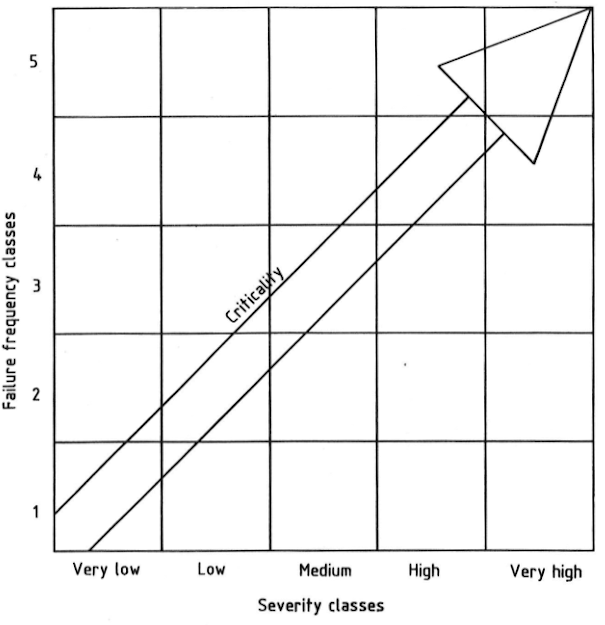
\includegraphics[width=\linewidth]{subfiles/imgs/fmea_criticality_grid.png}
  \caption{Criticality Grid}
        \label{fig:criticality_grid}
\end{figure}


\begin{figure}
        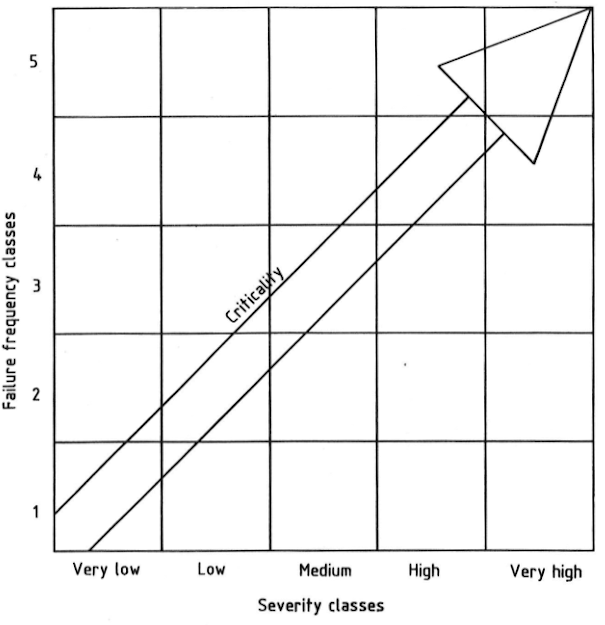
\includegraphics[width=\linewidth]{subfiles/imgs/fmea_criticality_grid.png}
  \caption{Criticality Grid}
        \label{fig:criticality_grid}
\end{figure}



\begin{figure}
	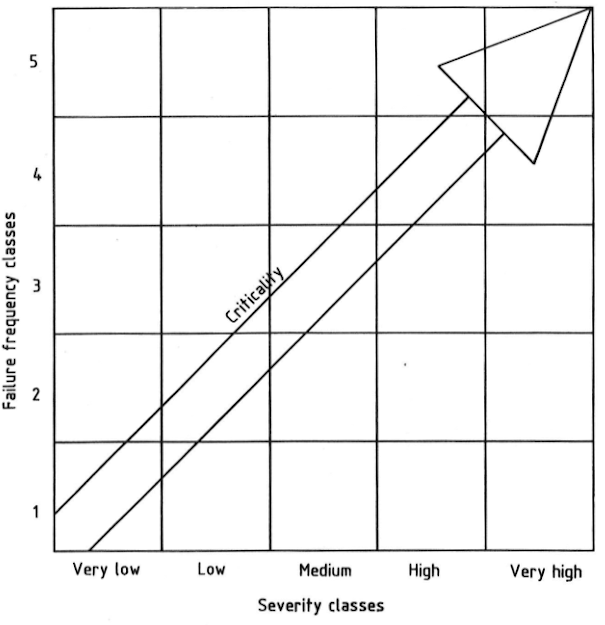
\includegraphics[width=\linewidth]{subfiles/imgs/fmea_criticality_grid.png}
  \caption{Criticality Grid}
	\label{fig:criticality_grid}
\end{figure}


\begin{figure}
	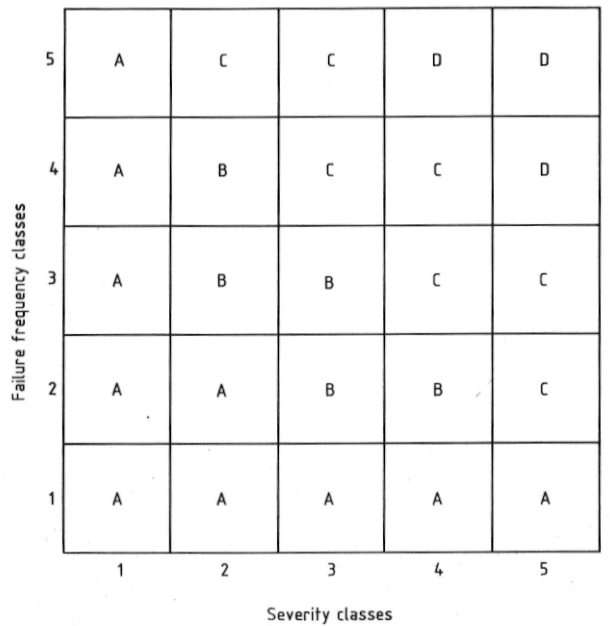
\includegraphics[width=\linewidth]{subfiles/imgs/fmea_criticality_matrix_with_bands.png}
  \caption{FMEA Criticality Matrix}
  \label{fig:criticality_matrix}
\end{figure}


\section{Supplementary Information}
\subsection{Establishment of Ground Rules}
\subsubsection{Levels of Analysis}

It is important to determine the level in the system that will be used for the analysis. For example, systems can be broken down into subsystems, replaceable units, or individual components (see figure 2). Basic principles for selecting the system levels for analysis depend on the results desired and the availability of design information. The following guidelines are useful.

\begin{enumerate}
\item The highest level within the system is selected from the design concept and specified output requirements.
\item The lowest level within the system at which the analysis is effective is that level for which information is available to establish definition and description of functions. The appropriate system level is influenced by previous experience. Less detailed analysis may be justified for a system based on a mature design, with good reliability, maintainability and safety record. Conversely, greater detail and a correspondingly lower system level is indicated for any newly designed system or a system with unknown reliability history.
\item The specified or intended maintenance and repair level may be a valuable guide in determining lower system levels.
\end{enumerate}






\subsection{Failure Modes}
Successful operation of a given system is subject to the performance of certain critical system elements. The key to evaluation of system performance is the identification of critical elements. The procedures for identifying failure modes, their causes, and effects can be effectively enhanced by the preparation of a list of failure modes anticipated in the light of the following:

\begin{enumerate}
\item The usage of the system;
\item The particular system element involved;
\item The mode of operation;
\item The pertinent operational specifications;
\item The time constraints;
\item The environment.
\end{enumerate}

In the FMEA, the definitions of failure modes, failure causes, and failure effects depend on the level of analysis. As the analysis progresses, the failure effects identified at the lower level may become failure modes at the higher level. Similarly, the failure modes at the lower level may become the failure causes at the higher level, and so on. A list of general failure modes is given in Table 1. Virtually every type of failure mode can be classified into one or more of these categories. However, these general failure mode categories are too broad in scope for definitive analysis; consequently, the list needs to be expanded to make the categories more specific as shown in Table 2. Failure modes such as those listed in Table 2 can describe the failure of any system element in sufficiently specific terms. When used in conjunction with performance specifications governing the inputs and outputs on the reliability block diagram, all potential failure modes can be identified and described. It should be noted that a given failure mode may have several causes.

\begin{table}[H]
\centering
\caption{Example set of general failure modes}
\label{tab:failure-modes}
\begin{tabular}{ll}
\hline
\textbf{Mode} & \textbf{Description} \\
\hline
1 & Failure during operation \\
\hline
2 & Failure to operate at a prescribed time \\
\hline
3 & Failure to cease operation at a prescribed time \\
\hline
4 & Premature operation \\
\hline
\end{tabular}
\end{table}

It is important that evaluation of all items within the system boundaries at the lowest practicable level is undertaken to identify all potential failure modes. Investigation to determine possible failure causes and also failure effects on subsystem and system function can then be undertaken. Item or equipment suppliers should identify the potential item failure modes within their products. To assist this function, typical failure mode data can be sought from the following areas:

\begin{enumerate}
\item For new items, reference can be made to other items with similar function and structure and to the results of tests performed on them under appropriate stress levels.
\item For items in use, in-service records and failure data may be consulted.
\item Potential failure modes can be deduced from functional and physical parameters typical of the operation of the item.
\end{enumerate}

It is important that item failure modes are not omitted for lack of data and that initial estimates are improved by test results and design progression. The FMEA should record the status of such estimates.

The identification of failure modes and, where necessary, the determination of remedial design actions, preventative quality assurance actions, or preventative maintenance actions is of prime importance. It is more important to identify and, if possible, design out modes than to know their rate of occurrence. When it is difficult to assign priorities, criticality analysis may be required.






\subsection{Failure Causes}
The possible causes associated with each possible failure mode should be identified and described. The causes of each failure mode are identified in order to estimate its probability of occurrence, to uncover secondary effects, and to devise recommended corrective action. Since a failure mode can have more than one cause, all potential independent causes for each failure mode need to be identified and described. The failure causes within the adjacent system levels should also be considered. The list given in Table B illustrates how a more specific definition of failure causes can be developed.

% Please add the following required packages to your document preamble:
% \usepackage{booktabs}
\begin{table}[]
\begin{tabular}{@{}llll@{}}
\toprule
\multicolumn{4}{l}{Example of an expanded tist of failure modes}                                                                                      \\ \midrule
1                          & Cracked/fractured                                 & 21                       & Binding/jamming                           \\
2                          & Distorted                                         & 22                       & Loose                                     \\
3                          & Undersize                                         & 23                       & Incorrect Adjustment                       \\
4                          & Oversize                                          & 24                       & Seized                                    \\
5                          & Fails to open                                     & 25                       & Worn                                      \\
6                          & Fails to close                                    & 26                       & Sticking                                  \\
7                          & Fail open                                         & 27                       & Overheated                                \\
8                          & Failed closed                                     & 28                       & False response                            \\
9                          & Internal leakage                                  & 29                       & Displaced                                 \\
10                         & External Leakage                                  & 30                       & Delayed operation                         \\
11                         & Fails to stop                                     & 31                       & Burned                                    \\
12                         & Fails to Start                                    & 32                       & Collapsed                                 \\
13                         & Corroded                                          & 33                       & Overloaded                                \\
14                         & Contaminated                                      & 34                       & Omitted                                   \\
15                         & Intermittent operation                            & 35                       & Incorrect assembly                        \\
16                         & Open circuit                                      & 36                       & Scored                                    \\
17                         & Short circuit                                     & 37                       & Noisy                                     \\
18                         & Out of tolerance (drifted)                        & 38                       & Arcing                                    \\
19                         & Fails to operate                                  & 39                       & Unstable                                  \\
20                         & Operates prematurely                              & 40                       & Chafed                                    \\
\multicolumn{4}{l}{\begin{tabular}[c]{@{}l@{}}NOTE: This list in an example only. The modes contained in the list\\  cannot be applied to all items and the list is not exhaustive\end{tabular}} \\ \bottomrule

\end{tabular}
\end{table}



\begin{table}[H]
\centering
\caption{Possible failure causes}
\label{tab:failure-causes2}
\begin{tabular}{|l|l|}
\hline
\textbf{Type} & \textbf{Examples} \\
\hline
Specification & Omitted statements, Erroneous statements, Support system failure \\
\hline
Design & Misapplication, Design error, Design omission, Support equipment failure \\
\hline
Manufacture & Omitted action, Erroneous action, Procedural error, Manufacturing equipment failure \\
\hline
Installation & Omitted action, Erroneous action, Procedural error, Installation equipment failure \\
\hline
Operation & Omitted action, Erroneous action, Procedural error, Off-line equipment failure \\
\hline
Maintenance & Omitted action, Erroneous action, Procedural error, Maintenance equipment failure \\
\hline
Environment & Temperature, Humidity, Vibration, Corrosion, Uncontrollable forces, Fire, Flood, Earthquake, Explosion \\
\hline
\end{tabular}
\end{table}

Note: This table is an example only. Different types and examples of failure causes may be required for different systems.


\subsection{Common-Cause (Common Mode) Failures}
In a reliability analysis, it is not sufficient to consider only random and independent failures. Some 'common-cause' (or 'common mode') failures (CCF) can occur that cause system performance degradation or failure through simultaneous deficiency in several system components, due to a single source such as design error or human error. A CCF is the result of an event that, because of logical dependencies, causes a coincidence of failure states in two or more components (excluding secondary failures caused by the effects of a primary failure).

CCFs can be analysed qualitatively using FMEA. As FMEA is a procedure to examine successively each failure mode and associated causes and also to identify all periodic tests, preventative maintenance measures, etc., it makes possible a study of all the causes which can induce potential CCF.

A check list developed from Table 3 may be used to identify in a detailed manner all possible causes which may induce CCF. A combination of several methods is useful in dealing with these failures: functional diversity, redundancies of different types, physical separation, tests, etc. Check lists, as above, may be used to examine the relevance and effectiveness of each method. The examination of preventative measures against CCF is usually considered to be outside the scope of FMEA, but this need not be the case.

\subsection{Human Factors}
Some systems have to be designed to cater for some human error, for example by providing mechanical interlocks on railway signals, and passwords for computer usage or data retrieval. Where such provisions exist in a system, the effect of failure of the provisions will depend on the type of error. Some modes of human error should also be considered for an otherwise fault-free system, to check the effectiveness of the provisions. Although incomplete, even a partial listing of these modes is beneficial for the identification of design and procedural deficiencies; the identification of all possible forms of human error would probably be impossible.

Many CCFs involve human factors. For example, incorrect maintenance of similar items can negate redundancy. To avoid this, material diversity in redundant elements is often introduced.

\subsection{Software Errors}
Malfunctions due to software errors or inadequacies will have effects whose significance will be determined by both hardware and software design. The postulation of such errors or inadequacies and the analysis of their effects is possible only to a limited extent. The effects upon associated hardware of possible errors in software may be estimated and the provision of fall-back arrangements either in software or hardware is often suggested by such analysis.

\subsection{Failure Detection Methods}
The methods for detection of the failure mode should be described. Failure modes other than the one being considered which give rise to an identical manifestation should be analysed and listed. The need for separate detection of failure of redundant elements during operation should be considered.

\subsection{Failure Effects}
\subsubsection{General}
A failure effect is the consequence of a failure mode in terms of the operation, function or status of a system (see 1.2.1). A failure effect may be caused by one or more failure modes of one or more items.

The consequences of each failure mode on system element operation, function, or status need to be identified, evaluated and recorded. Maintenance, preventive or corrective action to be taken in each case should be identified.

MISSING TABLE PAG 17

MISSING TABLE PAG 18

\section{1.9 Consequences of System Failure}

A system FMEA can be conducted independently, without referencing a specific application, and later adapted for project use. This is applicable to small assemblies, which can be considered as generic components (e.g., electronic amplifiers, electric motors, mechanical valves). However, it is more common to develop a project-specific FMEA and consider the particular consequences of system failure. It might be necessary to categorise the effects of failure on the system based on the consequences, such as fail-safe, fail-danger, repairable failure, non-repairable failure, mission degraded, mission failed, and effects on individuals, groups, or society in general.

The need to connect an FMEA to the ultimate consequence of system failure depends on the project and the relationship between the FMEA and other forms of analysis, such as fault trees.

\subsection{2.4.2 Information Required}

\subsubsection{2.4.2.1 General}

Company management should be aware that the success of FMEA (and FMECA) relies on the unrestricted availability of all relevant information to analysts and the active cooperation of the designer. Information in categories listed from 2.4.2.2 to 2.4.2.11 needs to be obtained.

\subsubsection{2.4.2.2 System Structure}

Information on system structure should include the following items:

\begin{enumerate}
\item[(a)] Different system elements with their characteristics, performances, roles, and functions;
\item[(b)] Logical connections between elements;
\item[(c)] Redundancy level and nature of the redundancies;
\item[(d)] Position and importance of the system within the whole facility (if possible);
\item[(e)] Inputs and outputs of the system;
\item[(f)] Changes in system structure for varying operational modes.
\end{enumerate}

Data related to functions, characteristics, and performances are required for all levels considered, up to the highest level.

\subsubsection{2.4.2.3 System Initiation, Operation, Control, and Maintenance}

The status of different operating conditions of the system should be specified, as well as the changes in the configuration or position of the system and its components during different operational phases. The minimum performances demanded of the system should be defined so that success and/or failure criteria can be clearly understood. Specific requirements, such as availability or safety, should be considered in terms of specified minimum levels of performance to be achieved and maximum levels of damage or harm to be accepted.

It is necessary to have accurate knowledge of:

\begin{enumerate}
\item[(a)] The duration of each task the system may be called upon to fulfil;
\item[(b)] The time interval between periodic tests;
\item[(c)] The time available for corrective action before serious consequences occur to the system;
\item[(d)] The entire facility, the environment, and/or the personnel, including interfaces and interactions with operators;
\item[(e)] Repair conditions, including corrective actions and the time, equipment, and/or personnel needed to achieve them;
\item[(f)] Operating procedures during system start-up, shut-down, and other operational transitions;
\item[(g)] Control during the operational phases;
\item[(h)] Preventative and/or corrective maintenance (see note);
\item[(i)] Procedures for routine testing, if employed.
\end{enumerate}

\textit{Note}: One of the uses of FMEA is to assist in the development of the maintenance strategy. However, if the latter has been pre-determined, information on maintenance facilities, equipment, and spares should be known for both preventative and corrective maintenance.

\subsubsection{2.4.2.4 System Environment}

The environmental conditions of the system should be specified, including ambient conditions and those created by other systems in the vicinity. The system should be delineated with respect to its relationships, dependencies, or interconnections with auxiliary or other systems and human interfaces.

At the design stage, these facts are usually not all known, and therefore approximations and assumptions will be needed. As the project progresses, the data will have to be augmented, and the FMEA modified to allow for new information or changed assumptions or approximations. Often, the FMEA will be helpful in defining the required conditions.

\textit{Note}: The FMEA should be updated for each design review milestone (see BS 5760: Part 1).

\subsubsection{2.4.2.5 Modelling}

FMEA requires some modelling of the system, i.e., a logical representation of the relevant information on the system (reliability block diagram or fault tree, etc.; see 2.4.2.9 and 2.4.2.10). Some assumptions may be made about the nature of failure modes and the seriousness of their consequences. For example, in safety studies, conservative hypotheses may have to be formed concerning the impact of certain failures on the system unless or until better information becomes available.

\subsection{2.4.2.6 Software}

An FMEA conducted on the hardware of a complex system may have repercussions on the software in the system. Thus, decisions about effects, criticality and conditional probabilities resulting from the FMEA may be dependent upon the software elements and their nature, sequence and timing. When this is the case, the interrelationships between hardware and software need to be clearly identified because any subsequent alteration or improvement of the software may modify the FMEA and the assessments derived from it. Approval of software development and change may be conditional upon a revision of the FMEA and the related assessments, e.g. software logic may be altered to improve safety at the expense of operational reliability.

\subsection{2.4.2.7 System boundary}

The definition of the system boundary is more likely to be influenced by design, source of supply, or commercial criteria rather than the optimum requirements of the FMEA. However, where it is possible to define the boundaries to facilitate the system FMEA and its integration with other related studies in the reliability program, such action is preferable. This is especially so if the system is functionally complex with multiple interconnections between items within the boundary and multiple outputs crossing the boundary. In such cases, it could be advantageous to define a study boundary from functional rather than hardware divisions to limit the number of input and output links to other systems. This would tend to reduce the number of system failure effects. Care should be taken to ensure that other systems or components outside the boundaries of the subject system are not forgotten, by explicitly stating that they are excluded from the particular study.

\subsection{2.4.2.8 Definition of the system's functional structure}

The analysis should be initiated by selecting the lowest level of interest (usually the part, circuit, or module level) at which sufficient information is available or at which it is judged that it needs to be obtained (by tests etc.) to ensure a reliable design. Thus new features of the design should be thoroughly investigated but old features under known stress levels can be incorporated into the analysis at a higher level. If the analysis starts at the lowest level, the various failure modes that can occur for each item at that level are tabulated. The corresponding failure effect for each, taken singly and in turn, is interpreted as a failure mode for consideration of the failure effect at the functional level immediately above. Successive iterations result in the identification of the failure effects, in relation to specific failure modes, at all necessary functional levels up to the system or highest level. The choice of breakdown level (which may vary for different areas of the system) requires a dependable and detailed knowledge of the failure modes of the elements. Apart from this requirement, it is neither possible nor desirable to set strict rules about the choice of the breakdown level. When quantitative results are required, the level chosen should be one at which it is possible to obtain adequate (and dependable) failure data on each failure mode or error mode, or to make reasonable identified assumptions of such failure rates. The analyst should investigate all aspects which might be important until satisfied they are not.

\subsection{2.4.2.9 Representation of system structure}

Symbolic representations of the system structure and operation, especially diagrams, can be used. Usually block diagrams are adopted, highlighting all the functions essential to the system. In the diagram, the blocks are linked together by lines which represent the inputs and outputs for each function. Usually, the nature of each function and each input needs to be precisely described. There may also be several diagrams to cover different phases of system operation. Generally, graphical presentations, including those closely related to analytical methods, like fault trees or cause-consequence diagrams, contribute to a better understanding of a system, its structure and its operation.

\subsection{Block Diagrams}

Diagrams showing the functional elements of the
system are necessary both for technical understanding of the functions and the subsequent analysis. The diagrams should display any series and redundant relationships among the elements and the functional inter-dependencies between them. This allows the functional failures to be tracked through the system. More than one diagram may be needed to display the alternative modes of system operation. Separate logic diagrams may be required for each operational mode. As a minimum, the block diagram should contain the following:

\begin{enumerate}
\item Breakdown of the system into major subsystems including functional relationships;
\item All appropriately labelled inputs and outputs and identification numbers by which each subsystem is consistently referenced;
\item All redundancies, alternative signal paths and other engineering features which provide 'fail-safe' measures.
\end{enumerate}

\subsection{Failure Significance and Compensating Provisions}

The relative significance of the failure should be recorded on the worksheet. Also recorded on the worksheet should be the identification and evaluation of any design features at a given system level for other provisions to prevent or reduce the effect of the failure mode. Thus the worksheet should clearly show the true behaviour of the equipment in the presence of an internal malfunction. Other provisions against failure which need to be recorded on the worksheet include the following:

\begin{enumerate}
\item Redundant items that allow continued operation if one or more elements fail;
\item Alternative means of operation;
\item Monitoring or alarm devices;
\item Any other means of permitting effective operation or limiting damage.
\end{enumerate}

During the design stage, the functional elements (hardware and software) of a piece of equipment may be rearranged or reconfigured to change its capability. Following this, the relevant failure modes should be re-examined before repeating the FMEA.
\end{document}
